
\subsection{Real robot testing and analysis} 

This section details the implementation of the proposed Complete Coverage Path Planning (CCP) algorithm on a real robot platform, addressing both scenarios with and without obstacles. The subsequent analysis of the experimental results is provided. The section is organized into two main parts: Experimental Setup and Results \& Analysis. 

\subsection{Experimental Setup} 

This subsection provides a comprehensive description of the real robot setup, emphasizing the experimental framework within which the tests are conducted.   

\vspace*{6mm}   


The real-world experiments were conducted using a specially designed robot platform equipped with a camera for weed detection and extraction, and a GPS module for localization. This robot is specifically engineered to operate in grass fields. The robot can be visualized in (\autoref{fig:real_robot}).   
\begin{figure}[htbp]
    \centering
    % 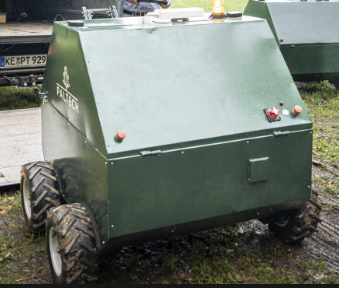
\includegraphics[width=\textwidth]{Images/real_robot/robot.png}
    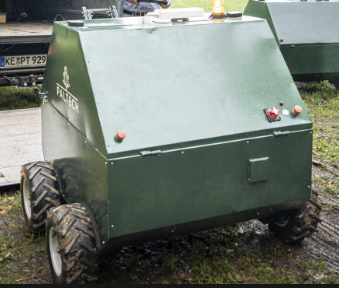
\includegraphics[width=0.5\textwidth]{Images/real_robot/robot.png}
    \caption{Real robot.}
    \label{fig:real_robot}
\end{figure}


\vspace*{6mm}   


To perform the tests on the real robot platform, a small region of the complete field was selected, and only the weed positions within this area were considered. Testing on the entire field was impractical due to its extensive size and the significant time required for complete coverage. Therefore, a smaller region was chosen for practical testing purposes and is demonstrated in the (\autoref{fig:field_region}). Additionally, complete coverage was not pursued due to time constraints. Instead, the robot was programmed to cover 42\% of the points, with the expectation that the robot would behave similarly even with full coverage. This assumption is based on the robot's ability to mimic its behavior in the simulation accurately. The selected region for experimentation and the specific points utilized for the tests are demonstrated in the (\autoref{fig:field_region}). 

% seleced field region.
\begin{figure}[H]
    \centering
    \begin{tabular}{ccc} 
        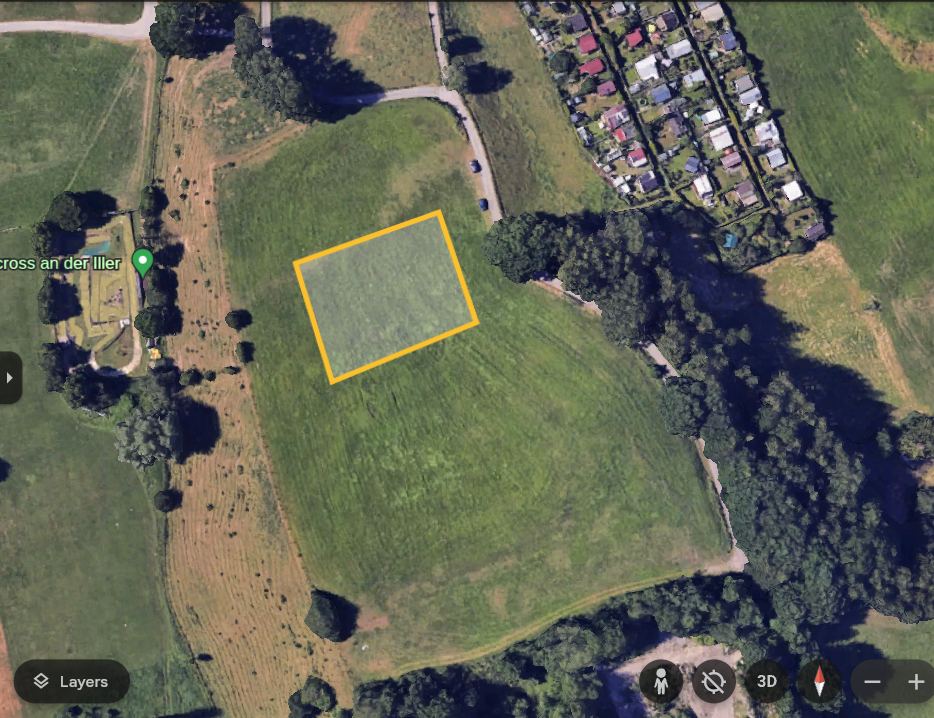
\includegraphics[height=46mm,width=0.4\textwidth]{Images/real_robot/field_with_region.png}
        & 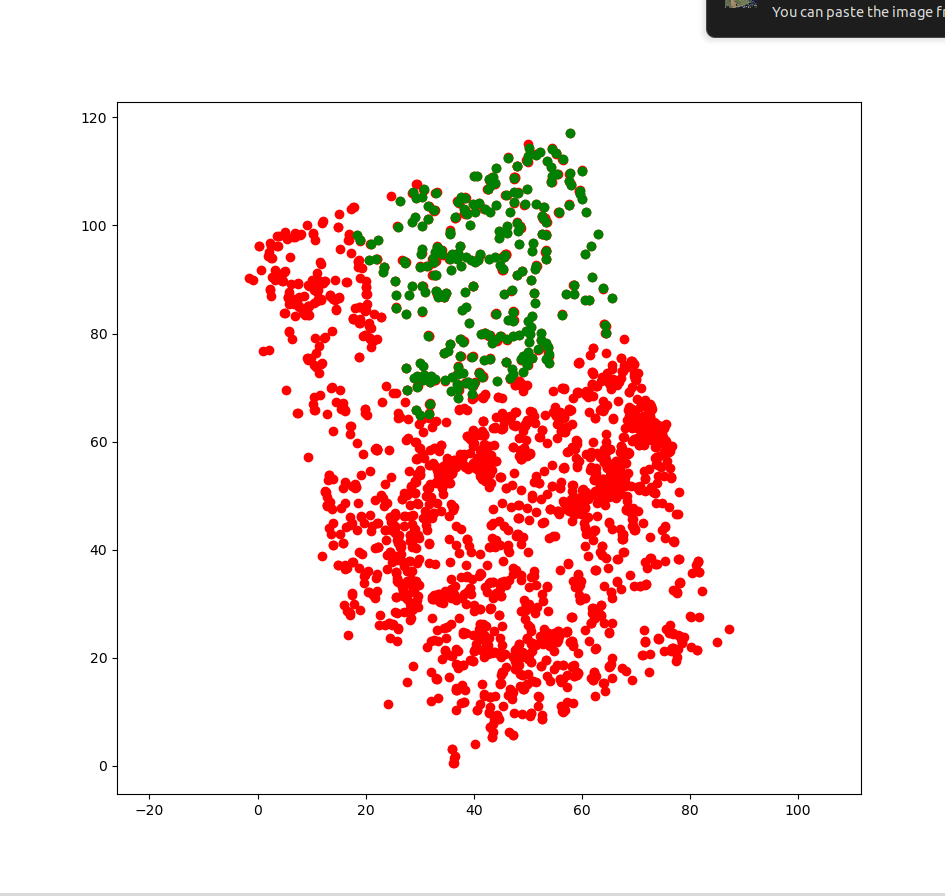
\includegraphics[height=46mm,width=0.4\textwidth]{Images/real_robot/field_region_points.png} 

    \end{tabular}
    \caption{Selected field region.\label{fig:field_region}} 
\end{figure}



\vspace*{6mm}   


Apart from these adjustments, all the robot constraints and parameters were kept consistent with those discussed in the simulation setup. Two experimental cases were considered: one without obstacles and the other with obstacles. For the scenario involving obstacles, two polygonal obstacles (one concave and one convex) were introduced. The figures below depict both experimental scenarios. 


\vspace*{6mm}   


The objective of demonstrating the CCP algorithm on a real robot platform is twofold: to showcase the alignment between the simulated global trajectory and the actual trajectory followed by the robot, and to evaluate the algorithm's effectiveness in weed removal. Specifically, the analysis focuses on how many weeds the robot successfully removes compared to the number planned by the global planner. Since the robot relies on its local planner, any deviation from the global planner's trajectory could result in missed weeds or the coverage of additional, unintended weed points.

\vspace*{6mm}   


This approach aims to highlight the practical applicability and robustness of the CCP algorithm in real-world agricultural settings, emphasizing its ability to adapt to various environmental conditions and obstacles while maintaining efficient operational performance.

\vspace*{6mm}   


\textbf{Real Robot Results and Analysis:}    

Initially, the real-world experiment was conducted on the first case without obstacles. Given that only 42\% coverage was used to demonstrate the results on the real robot, the global trajectory obtained from the simulation is depicted below. After executing the test on the real robot in the field, the actual path followed by the robot using the local planner is provided in the subsequent figure.

\textbf{Global trajectory}

\textbf{Local trajectory}


\vspace*{6mm}   


The number of weeds planned by the local planner to be extracted was X, and the number of weeds actually removed by the robot was Y. The alignment between the global and local trajectories can be visualized in the figure below. To quantify this alignment, the absolute trajectory error (ATE) and relative pose error (RPE) were calculated, metrics commonly used in visual odometry literature. The ATE was x, and the RPE was y. Additional results, if available, can be visualized in the figure below.

\textbf{Both trajectories on same  plot} 


\vspace*{6mm}   


Similarly, the same procedure was performed for the second case with obstacles. The global trajectory from the simulation and the local trajectory from the real robot are shown below. In this scenario, the number of weeds planned for extraction by the local planner was X, and the number of weeds actually removed by the robot was Y. The alignment between the two trajectories is illustrated in the figure below. The absolute trajectory error was x, and the relative pose error was y. Any additional results obtained are also visualized in the figure below.

\textbf{Global trajectory}

\textbf{Local trajectory}

\textbf{Both trajectories on same  plot} 


\vspace*{6mm}   


\textbf{Analysis: }

From the results, it can be summarized that the local planner (real robot) closely follows the global planner, demonstrating the accuracy of the global planner in modeling the robot's constraints in a manner that aligns well with the local planner. A key focus is the comparison between the number of weeds planned for extraction and the number of weeds actually removed. Ideally, these numbers should match as closely as possible, depending on the alignment between the local and global trajectories.

\vspace*{6mm}   

If the robot accurately follows the global trajectory, it will cover and extract all the planned weeds. Conversely, if there is a deviation, the robot may fail to extract some of the planned weeds and instead remove others that were not targeted. These additional weeds would have been covered in subsequent passes, and the missed weeds would remain uncovered, resulting in incomplete coverage.

\vspace*{6mm}   

Thus, the alignment between the global and local trajectories is crucial and can be assessed using the absolute trajectory error and relative pose error. These trajectory error metrics indirectly indicate the efficiency of the algorithm and the alignment between the global and local planners. Therefore, complete coverage is more likely if the trajectory deviation is minimal, whereas greater deviation compromises coverage completeness, leaving some weed points untreated.

\vspace*{6mm}   

By ensuring minimal deviation, the proposed CCP algorithm can achieve efficient and effective coverage, thus validating its applicability in real-world agricultural scenarios. The detailed analysis underscores the importance of trajectory alignment in achieving the desired operational outcomes.

\vspace*{6mm}   
